%\documentclass[hyperref={pdfpagelabels=false},slidetop,9pt]{beamer}
\documentclass[slidetop,8pt]{beamer}
\usepackage[T1]{fontenc}
\usepackage[utf8]{inputenc}
\newcommand{\id}{71}
\newcommand{\nom}{Théorie des mécanismes}
\newcommand{\sequence}{04}
\newcommand{\nomsequence}{Liaisons entre les solides}
\newcommand{\num}{02}
\newcommand{\type}{KH}
\newcommand{\descrip}{Liaisons équivalentes, hyperstatisme, liaisons en série et en parallèle, théorie des graphes}
\newcommand{\competences}{B2-12: Proposer une modélisation des liaisons avec leurs caractéristiques géométriques. \\ &  B2-13: Proposer un modèle cinématique paramétré à partir d'un système réel, d'une maquette numérique ou d'u \\ &  B2-17: Simplifier un modèle de mécanisme. \\ &  B2-18: Modifier un modèle pour le rendre isostatique. \\ &  C1-04: Proposer une démarche permettant d'obtenir une loi entrée-sortie géométrique.  \\ &  C2-05: Caractériser le mouvement d'un repère par rapport à un autre repère. \\ &  C2-06: Déterminer les relations entre les grandeurs géométriques ou cinématiques. }
\newcommand{\nbcomp}{7}
\newcommand{\systemes}{}
\newcommand{\systemesnum}{}
\newcommand{\systemessansaccent}{}
\newcommand{\ilot}{2}
\newcommand{\ilotstr}{02}
\newcommand{\dossierilot}{\detokenize{Ilot_02 }}

\usepackage{etex}
\usepackage{tikz}
\usepackage[european]{circuitikz}
\usepackage{pgf}
\usepackage[all]{xy}
\usepackage{pgfpages}
\usepackage{graphbox}
\usepackage{pdfpages}
%\usepackage[adobe-utopia]{mathdesign}
\usepackage{ifthen}
\usepackage{cancel}
\usepackage{framed}
\usepackage{subfig}
\usepackage{tabularx}
\usepackage{setspace}
\usepackage{soul}
\usepackage{schemabloc}
\usepackage{eqnarray}
\usepackage[dot, phantomtext]{dashundergaps}
\usepackage{media9}
\usepackage{multimedia}
\usepackage{textcomp}
\usefonttheme[onlymath]{serif}

\author{Renaud Costadoat}
\institute{Lycée Dorian}

\usepackage{multido}
\usepackage{multirow}
\usepackage{multicol} % Portions de texte en colonnes
\usepackage{flafter}%floatants après la référence

\usepackage{color}
\usepackage{xcolor}
\usepackage{colortbl}

\usepackage[gen]{eurosym}
\usepackage{tikz}
%\usepackage{pstricks,pst-node,pst-tree,pst-solides3d}
\usepackage{lmodern}
\usepackage[francais]{babel}
\usepackage{pslatex}
\usetheme{renaud}
\usepackage{times}
\usepackage[frenchmath]{newtxsf} % for sans serif symbols
\renewcommand{\familydefault}{\sfdefault}
%\usepackage{amsfonts}
%\usepackage{amsmath}
%\usepackage{mathastext}
\usepackage{verbatim}
\usepackage{moreverb}
%\usetikzlibrary{arrows,shapes}
\usepackage{graphicx}
\usepackage{psfrag}
\usepackage{wrapfig}
\usepackage{etoolbox}

\definecolor{gris25}{gray}{0.75}
\definecolor{bleu}{RGB}{18,33,98}
\definecolor{bleuf}{RGB}{42,94,171}
\definecolor{bleuc}{RGB}{231,239,247}
\definecolor{rougef}{RGB}{185,18,27}
\definecolor{rougec}{RGB}{255,188,204}%255,230,231
\definecolor{vertf}{RGB}{103,126,82}
\definecolor{vertc}{RGB}{220,255,191}

\setlength\parindent{24pt}
\parskip 7.2pt
\parindent 8pt

\newenvironment{rem}[1][\hsize]%
{%
    \def\FrameCommand
   {%
\rotatebox{90}{\textit{\textsf{Remarque}}} 
       {\color{bleuf}\vrule width 3pt}%
       \hspace{0pt}%must no space.
       \fboxsep=\FrameSep\colorbox{bleuc}%
  }%
    \MakeFramed{\hsize#1\advance\hsize-\width\FrameRestore}%
}%
{\endMakeFramed}%


\newenvironment{savoir}[1][\hsize]%
{%
    \def\FrameCommand
    {%
\rotatebox{90}{\textit{\textsf{Savoir}}} 
        {\color{bleuf}\vrule width 3pt}%
        \hspace{0pt}%must no space.
        \fboxsep=\FrameSep\colorbox{bleuc}%
    }%
    \MakeFramed{\hsize#1\advance\hsize-\width\FrameRestore}%
}%
{\endMakeFramed}%

\newenvironment{prob}[1][\hsize]%
{%
    \def\FrameCommand%
    {%
\rotatebox{90}{\textit{\textsf{Problematique}}} 
        {\color{rougef}\vrule width 3pt}%
        \hspace{0pt}%must no space.
        \fboxsep=\FrameSep\colorbox{rougec}%
    }%
    \MakeFramed{\hsize#1\advance\hsize-\width\FrameRestore}%
}%
{\endMakeFramed}%

\newenvironment{obj}[1][\hsize]%
{%
    \def\FrameCommand%
    {%
\rotatebox{90}{\textit{\textsf{Objectif}}} 
        {\color{vertf}\vrule width 3pt}%
        \hspace{0pt}%must no space.
        \fboxsep=\FrameSep\colorbox{vertc}%
    }%
    \MakeFramed{\hsize#1\advance\hsize-\width\FrameRestore}%
}%
{\endMakeFramed}%

\newenvironment{defi}[1][\hsize]%
{%
    \def\FrameCommand%
    {%
\rotatebox{90}{\textit{\textsf{Definition}}} 
        {\color{bleuf}\vrule width 3pt}%
        \hspace{0pt}%must no space.
        \fboxsep=\FrameSep\colorbox{rougec}%
    }%
    \MakeFramed{\hsize#1\advance\hsize-\width\FrameRestore}%
}%
{\endMakeFramed}%


\newenvironment{hypo}[1][\hsize]%
{%
    \def\FrameCommand%
    {%
\rotatebox{90}{\textit{\textsf{Hypothèse\\}}} 
        {\color{bleuf}\vrule width 3pt}%
        \hspace{0pt}%must no space.
        \fboxsep=\FrameSep\colorbox{bleuc}%
    }%
    \MakeFramed{\hsize#1\advance\hsize-\width\FrameRestore}%
}%
{\endMakeFramed}%


\newenvironment{prop}[1][\hsize]%
{%
    \def\FrameCommand%
    {%
\rotatebox{90}{\textit{\textsf{Propriété}}} 
        {\color{bleuf}\vrule width 3pt}%
        \hspace{0pt}%must no space.
        \fboxsep=\FrameSep\colorbox{bleuc}%
    }%
    \MakeFramed{\hsize#1\advance\hsize-\width\FrameRestore}%
}%
{\endMakeFramed}%

\newenvironment{props}[1][\hsize]%
{%
    \def\FrameCommand%
    {%
\rotatebox{90}{\textit{\textsf{Propriétés}}} 
        {\color{bleuf}\vrule width 3pt}%
        \hspace{0pt}%must no space.
        \fboxsep=\FrameSep\colorbox{bleuc}%
    }%
    \MakeFramed{\hsize#1\advance\hsize-\width\FrameRestore}%
}%
{\endMakeFramed}%

\newenvironment{exemple}[1][\hsize]%
{%
    \def\FrameCommand%
    {%
\rotatebox{90}{\textit{\textsf{Exemple}}} 
        {\color{vertf}\vrule width 3pt}%
        \hspace{0pt}%must no space.
        \fboxsep=\FrameSep\colorbox{vertc}%
    }%
    \MakeFramed{\hsize#1\advance\hsize-\width\FrameRestore}%
}%
{\endMakeFramed}%

\newenvironment{resultat}[1][\hsize]%
{%
    \def\FrameCommand%
    {%
\rotatebox{90}{\textit{\textsf{Résultat}}} 
        {\color{rougef}\vrule width 3pt}%
%        {\color{bleuf}\vrule width 3pt}%
        \hspace{0pt}%must no space.
        \fboxsep=\FrameSep\colorbox{rougec}%
    }%
    \MakeFramed{\hsize#1\advance\hsize-\width\FrameRestore}%
}%
{\endMakeFramed}%

\newenvironment{methode}[1][\hsize]%
{%
    \def\FrameCommand%
    {%
\rotatebox{90}{\textit{\textsf{Méthode\\}}} 
        {\color{rougef}\vrule width 3pt}%
        \hspace{0pt}%must no space.
        \fboxsep=\FrameSep\colorbox{rougec}%
    }%
    \MakeFramed{\hsize#1\advance\hsize-\width\FrameRestore}%
}%
{\endMakeFramed}%

\newenvironment{theo}[1][\hsize]%
{%
    \def\FrameCommand%
    {%
\rotatebox{90}{\textit{\textsf{Théorème\\}}} 
        {\color{rougef}\vrule width 3pt}%
        \hspace{0pt}%must no space.
        \fboxsep=\FrameSep\colorbox{rougec}%
    }%
    \MakeFramed{\hsize#1\advance\hsize-\width\FrameRestore}%
}%
{\endMakeFramed}%

\newenvironment{warn}[1][\hsize]%
{%
    \def\FrameCommand%
    {%
\rotatebox{90}{\textit{\textsf{Attention\\}}} 
        {\color{rougef}\vrule width 3pt}%
        \hspace{0pt}%must no space.
        \fboxsep=\FrameSep\colorbox{rougec}%
    }%
    \MakeFramed{\hsize#1\advance\hsize-\width\FrameRestore}%
}%
{\endMakeFramed}%

% \usepackage{pstricks}
%\usepackage{minitoc}
% \setcounter{minitocdepth}{4}

\setcounter{tocdepth}{2}

% \mtcselectlanguage{french} 

%\usepackage{draftcopy}% "Brouillon"
% \usepackage{floatflt}
\usepackage{psfrag}
%\usepackage{listings} % Permet d'insérer du code de programmation
\renewcommand{\baselinestretch}{1.2}

% Changer la num�rotation des figures :
% ------------------------------------
% \makeatletter
% \renewcommand{\thefigure}{\ifnum \c@section>\z@ \thesection.\fi
%  \@arabic\c@figure}
% \@addtoreset{figure}{section}
% \makeatother
 


%%%%%%%%%%%%
% Définition des vecteurs %
%%%%%%%%%%%%
 \newcommand{\vect}[1]{\overrightarrow{#1}}

%%%%%%%%%%%%
% Définition des torseusr %
%%%%%%%%%%%%

 \newcommand{\torseur}[1]{%
\left\{{#1}\right\}
}

\newcommand{\torseurcin}[3]{%
\left\{\mathcal{#1} \left(#2/#3 \right) \right\}
}

\newcommand{\torseurstat}[3]{%
\left\{\mathcal{#1} \left(#2\rightarrow #3 \right) \right\}
}

 \newcommand{\torseurc}[8]{%
%\left\{#1 \right\}=
\left\{
{#1}
\right\}
 = 
\left\{%
\begin{array}{cc}%
{#2} & {#5}\\%
{#3} & {#6}\\%
{#4} & {#7}\\%
\end{array}%
\right\}_{#8}%
}

 \newcommand{\torseurcol}[7]{
\left\{%
\begin{array}{cc}%
{#1} & {#4}\\%
{#2} & {#5}\\%
{#3} & {#6}\\%
\end{array}%
\right\}_{#7}%
}

 \newcommand{\torseurl}[3]{%
%\left\{\mathcal{#1}\right\}_{#2}=%
\left\{%
\begin{array}{l}%
{#1} \\%
{#2} %
\end{array}%
\right\}_{#3}%
}

 \newcommand{\vectv}[3]{%
\vect{V\left( {#1} \in {#2}/{#3}\right)}
}


\newcommand{\vectf}[2]{%
\vect{R\left( {#1} \rightarrow {#2}\right)}
}

\newcommand{\vectm}[3]{%
\vect{\mathcal{M}\left( {#1}, {#2} \rightarrow {#3}\right)}
}


 \newcommand{\vectg}[3]{%
\vect{\Gamma \left( {#1} \in {#2}/{#3}\right)}
}

 \newcommand{\vecto}[2]{%
\vect{\Omega\left( {#1}/{#2}\right)}
}

\newcommand{\reponse}[1][4]
{
\multido{}{#1}
{
\begin{center}
\makebox[0.9\linewidth]{\dotfill} \end{center}
}}


% }$$\left\{\mathcal{#1} \right\}_{#2} =%
% \left\{%
% \begin{array}{c}%
%  #3 \\%
%  #4 %
% \end{array}%
% \right\}_{#5}}


%  ------------------------------------------
% | Modification du formatage des sections : | 
%  ------------------------------------------

% Grands titres :
% ---------------

\newcommand{\titre}[1]{%
\begin{center}
      \bigskip
      \rule{\textwidth}{1pt}
      \par\vspace{0.1cm}
      
      \textbf{\large #1}
      \par\rule{\textwidth}{1pt}
    \end{center}
    \bigskip
  }

% Supprime le numéro du chapitre dans la numérotation des sections:
% -----------------------------------------------------------------
\makeatletter
\renewcommand{\thesection}{\@arabic\c@section}
\makeatother


% \titleformat{\chapter}[display]
% {\normalfont\Large\filcenter}
% {}
% {1pc}
% {\titlerule[1pt]
%   \vspace{1pc}%
%   \Huge}[\vspace{1ex}%
% \titlerule]


%%%% Chapitres Comme PY Pechard %%%%%%%%%
% numéro du chapitre
\DeclareFixedFont{\chapnumfont}{OT1}{phv}{b}{n}{80pt}
% pour le mot " Chapitre "
\DeclareFixedFont{\chapchapfont}{OT1}{phv}{m}{it}{40pt}
% pour le titre
\DeclareFixedFont{\chaptitfont}{T1}{phv}{b}{n}{25pt}

\definecolor{gris}{gray}{0.75}
\setbeamertemplate{section in toc}[sections numbered]

\newlength{\RoundedBoxWidth}
\newsavebox{\GrayRoundedBox}
\newenvironment{GrayBox}[1][\dimexpr\textwidth-4.5ex]%
   {\setlength{\RoundedBoxWidth}{\dimexpr#1}
    \begin{lrbox}{\GrayRoundedBox}
       \begin{minipage}{\RoundedBoxWidth}}%
   {   \end{minipage}
    \end{lrbox}
    \begin{center}
    \begin{tikzpicture}%
       \draw node[draw=bleuf,fill=bleuc,rounded corners,%
             inner sep=2ex,text width=\RoundedBoxWidth]%
             {\usebox{\GrayRoundedBox}};
    \end{tikzpicture}
    \end{center}}
    
\ifdef{\prive}{\pgfpagesuselayout{2 on 1}[a4paper,border shrink=0mm]}
\ifdef{\prive}{\setbeamertemplate{navigation symbols}{}}
\setbeamertemplate{itemize item}[ball]
%\setbeamertemplate{blocks}[rounded]%[shadow=true]
\setbeamercolor{block title}{fg=white,bg=grisf}        % titre block normal 
\setbeamercolor{block body}{fg=grisf,bg=grisc!50}      % corps block normal
\setbeamercolor{block body alerted}{fg=white,bg=warning}   % idem pour un block alerte

\title{\nom}
\date{S\sequence \ - \type\num}

\begin{document}
\shorthandoff{:!}
\bibliographystyle{abbrvnat-fr}

\usebackgroundtemplate%
{%
    \centering
\includegraphics[width=\paperwidth]{/home/renaud/Documents/Renaud/GitHub/Sciences-Ingenieur/img/fond2}%
}

{
\setbeamertemplate{navigation symbols}{}
\setbeamertemplate{headline}[pagetitre]
\setbeamertemplate{footline}[pagetitre]
\usebackgroundtemplate{\centering
\includegraphics[width=\paperwidth]{/home/renaud/Documents/Renaud/GitHub/Sciences-Ingenieur/img/fond}}
\frame{\titlepage}
}



\section{Définitions}

 \ifdef{\public}{\begin{frame}
\frametitle{Table des matières}
\tableofcontents[currentsection]
\end{frame}}{}

{\frame{
\frametitle{Les systèmes asservis}

\begin{savoir}

Vous êtes capables :

\begin{itemize}
 \item De décrire un système à l'aide des chaînes d'énergie et d'information,
 \item De décrire structurellement un système,
 \item De modéliser un asservissement par une fonction de transfert.
\end{itemize}
\end{savoir}

\begin{prob}

Vous devez être capables
\begin{itemize}
 \item De modéliser la structure d'un asservissement.
\end{itemize}
\end{prob}
}}

{\frame{
\frametitle{Représentation par schéma-blocs}

\begin{itemize}
 \item Un SLCI est généralement décrit par un système d'équations différentielles.
 \item Pour traduire le système de relations algébriques dans ce domaine de façon lisible, une représentation graphique est utilisée, il s'agit du \textbf{schéma bloc}. 
\end{itemize}

\begin{center}
 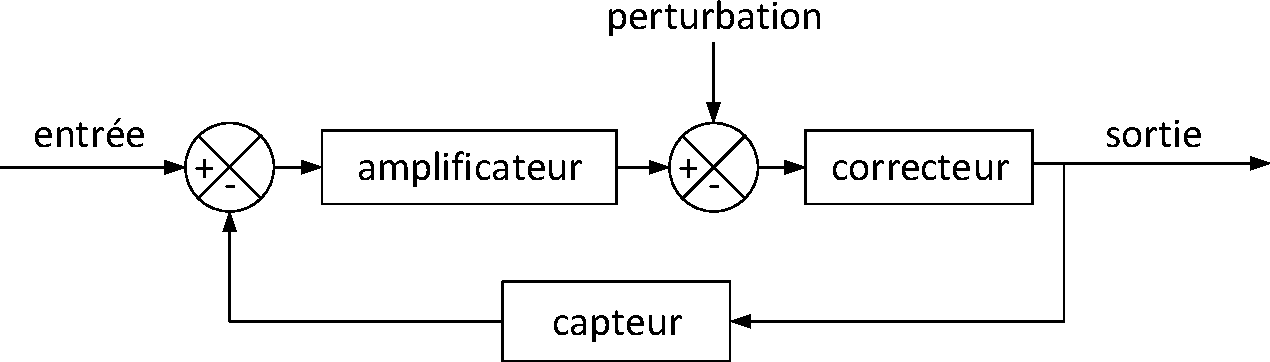
\includegraphics[width=0.8\linewidth]{img/fig1}
\end{center}
}}

{\frame{
\frametitle{Représentation par schéma-blocs}

\begin{itemize}
 \item Chaque \og boite \fg traduit une relation de causalité entre une grandeur d'entrée et une grandeur de sortie,
 \item Cette relation de causalité se traduit par une \textbf{fonction de transfert}.
\end{itemize}

Le schéma bloc suivant présente ces fonctions de transfert:

\begin{center}
 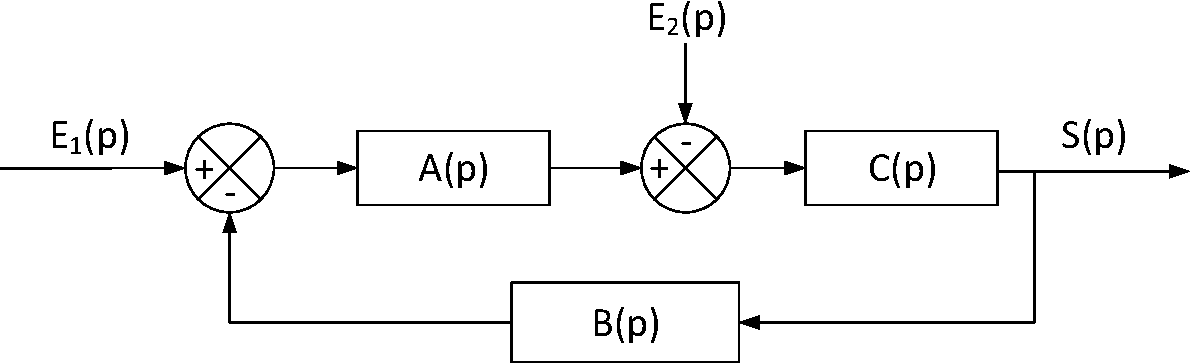
\includegraphics[width=0.7\linewidth]{img/fig2}
\end{center}
}}

{\frame{
\frametitle{Représentation par schéma-blocs}

\textbf{Les blocs}

\begin{center}
 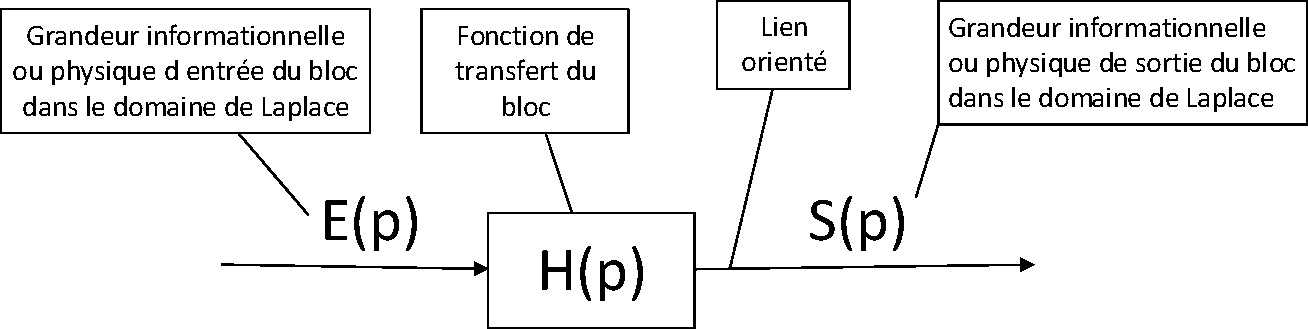
\includegraphics[width=0.7\linewidth]{img/fig3}
\end{center}

\begin{minipage}[t]{0.5\linewidth}
\textbf{Les comparateurs}

\begin{center}
 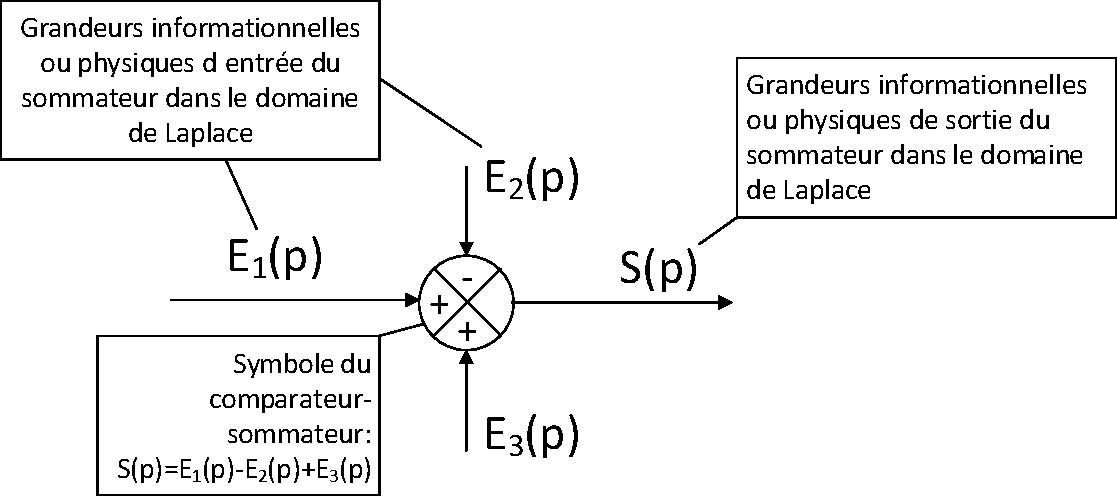
\includegraphics[width=0.9\linewidth]{img/fig4}
\end{center}
\end{minipage}\hfill
\begin{minipage}[t]{0.4\linewidth}
\textbf{Les points de prélèvement}

\begin{center}
 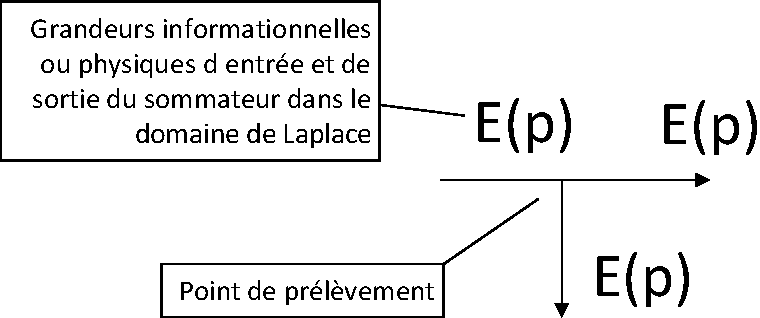
\includegraphics[width=0.9\linewidth]{img/fig5}
\end{center}
\end{minipage}
}}

{\frame{
\frametitle{Représentation par schéma-blocs}

\textbf{Fonction de transfert d'une chaîne directe}

La fonction de transfert de la chaîne est le produit des fonctions de transfert de chaque élément.

\begin{center}
 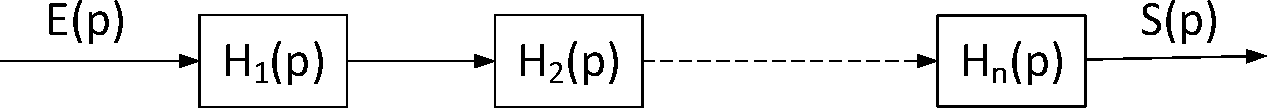
\includegraphics[width=0.5\linewidth]{img/fig6}
\end{center}

$H(p)=\dfrac{S(p)}{E(p)}=H_1(p).H_2(p)...H_n(p)$

\textbf{Fonction de transfert de chaînes en parallèle}

La fonction de transfert de la chaîne est la somme des fonctions de transfert de chaque élément.


\begin{center}
\begin{minipage}{0.49\linewidth}
 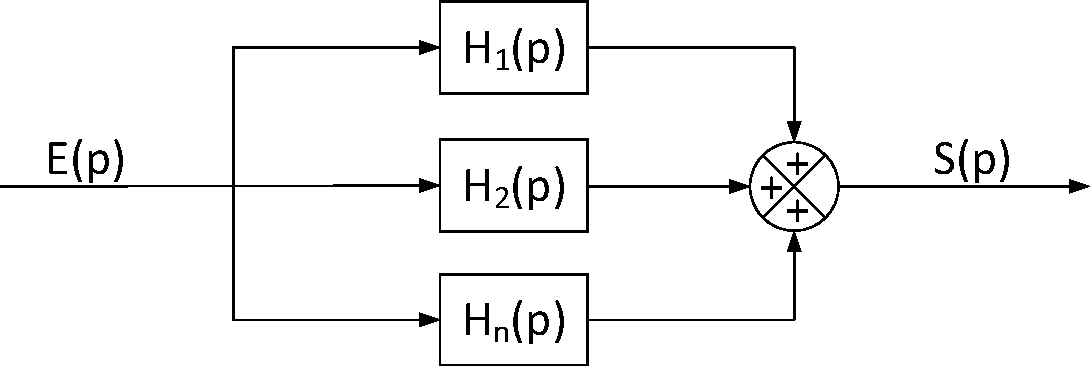
\includegraphics[width=0.8\linewidth]{img/fig7}
\end{minipage}\hfill
\begin{minipage}{0.49\linewidth}
$H(p)=\dfrac{S(p)}{E(p)}=\sum\limits_{i=1}^n H_i(p)$
\end{minipage}
\end{center}
}}

{\frame{
\frametitle{Représentation par schéma-blocs}

\textbf{Déplacement d'un point de prélèvement}

\begin{center}
 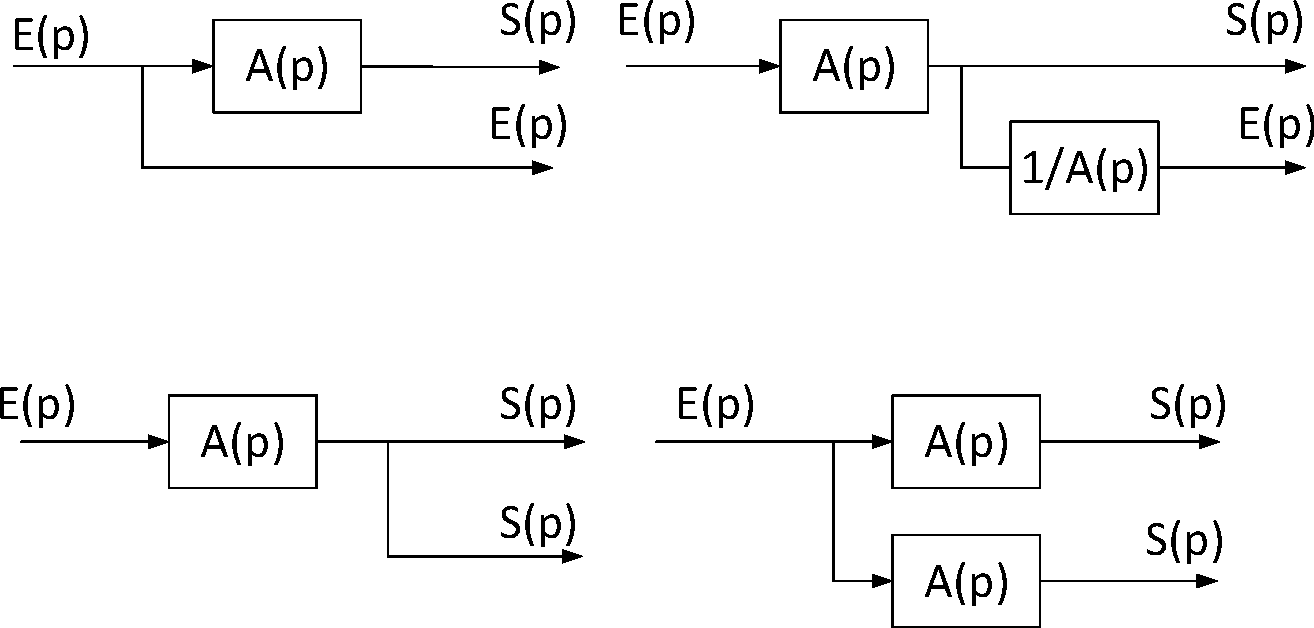
\includegraphics[width=0.5\linewidth]{img/fig8}
\end{center}

\textbf{Déplacement d'un sommateur}

\begin{center}
 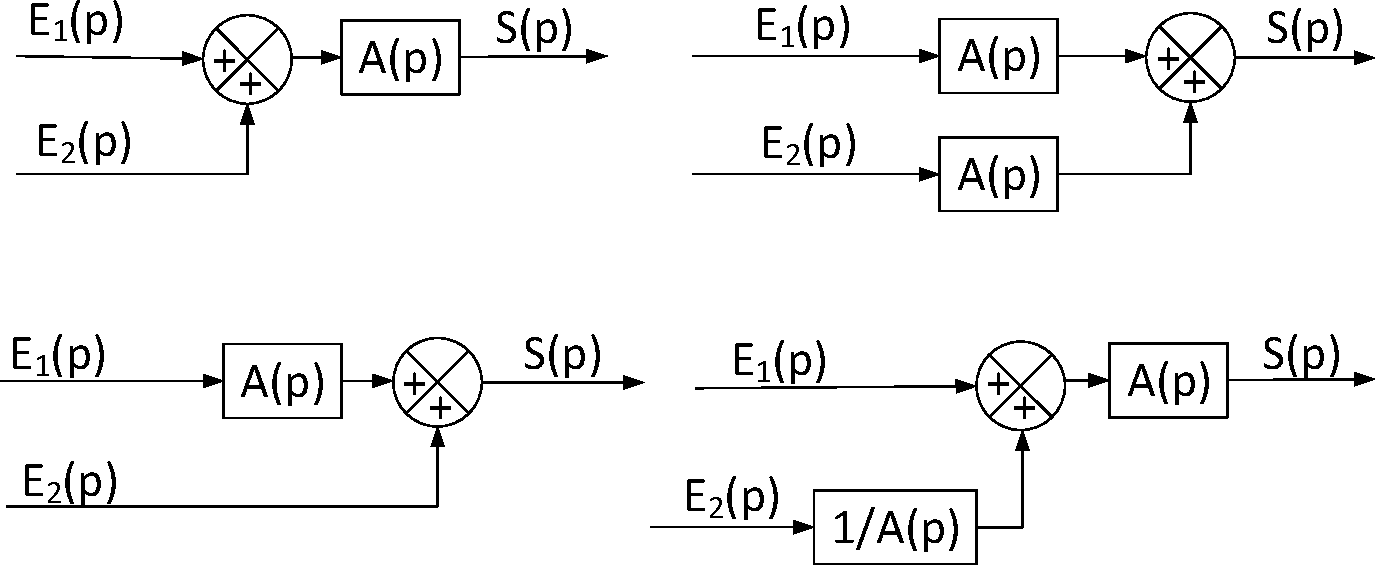
\includegraphics[width=0.5\linewidth]{img/fig9}
\end{center}
}}


{\frame{
\frametitle{Le système asservi}

\begin{defi}
Un \textbf{système asservi}, ou un asservissement, est un système capable d'élaborer de manière autonome sa grandeur de commande à partir d'une valeur de consigne et d'une mesure de la réponse avec un capteur.
\end{defi}

\begin{center}
 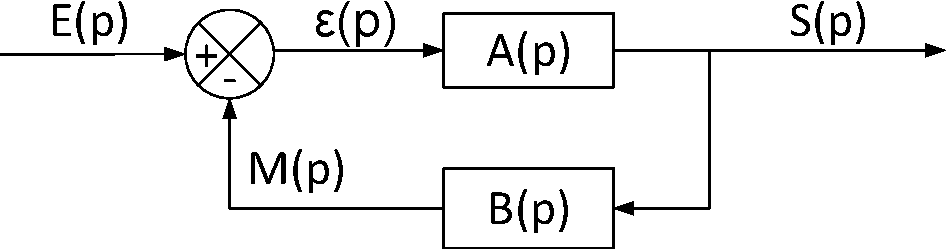
\includegraphics[width=0.4\linewidth]{img/fig10}
\end{center}

\begin{itemize}
 \item $E(p)$ est la grandeur de \textbf{Consigne},
 \item $S(p)$ celle de \textbf{Sortie},
 \item $M(p)$ est le \textbf{Mesurande} (image) de la sortie par la chaîne d'acquisition,
 \item $\epsilon(p)$ est l’\textbf{Écart} à la sortie du comparateur, qui permet d'établir la \textbf{Commande}.
\end{itemize}
}}

{\frame{
\frametitle{FTBO et FTBF}
\textbf{Fonction de Transfert en Boucle Ouverte (F.T.B.O.)}

\begin{defi}
 \begin{itemize}
  \item La FTBO est définie par: $FTBO(p)=\dfrac{M(p)}{\epsilon(p)}$
  \item Sa valeur est: $FTBO(p)=A(p).B(p)$
 \end{itemize}
\end{defi}

\textbf{Fonction de Transfert en Boucle Fermée (F.T.B.F.)}

\begin{defi}
 \begin{itemize}
  \item La FTBF est définie par: $FTBF(p)=\dfrac{S(p)}{E(p)}$
  \item Sa valeur est: $FTBF(p)=\dfrac{A(p)}{1+A(p).B(p)}$
 \end{itemize}
\end{defi}
}}

{\frame{
\frametitle{Rapidité et précision en réponse à un échelon}

\textbf{Rapidité}

\begin{itemize}
 \item L'étude de la rapidité du système s'effectue à l'aide de la notion de temps de réponse à 5\%. C'est le temps à partir duquel la réponse temporelle $s(t)$ est telle que : $\mathbf{0,95.s(+\infty)\leq s(t)\leq 1,05.s(+\infty)}$,
 \item En supposant que l'entrée $e(t)$ est un échelon unitaire, la réponse indicielle (la réponse à cet échelon unitaire) à l'aide de la méthode de Laplace est : $e(t)=u(t)\rightarrow E(p)=\dfrac{1}{p}$,
 \item Cela permet de déterminer la sortie à l'aide de la FTBF du système car les conditions initiales sont supposées nulles. 
$S(p)=FTBF(p).E(p)$, avec $FTBF(p)=\dfrac{A(p)}{1+FTBO(p)}$,
 \item La réponse temporelle dépend donc de la nature de la FTBO (Classe, ordre, gain,...).
\end{itemize}
}}

{\frame{
\frametitle{Rapidité et précision en réponse à un échelon}

1\up{er} cas: La FTBO est de classe 0 et d'ordre 1: $FTBO(p)=\dfrac{K}{1+\tau.p}$.

Dans ce cas, la FTBF est:

\begin{center}
$FTBF(p)=\dfrac{A(p)}{1+\dfrac{K}{1+\tau.p}}=\dfrac{A(p).(1+\tau.p)}{(1+K)+\tau.p}=\dfrac{\dfrac{A(p).(1+\tau.p)}{1+K}}{1+\dfrac{\tau}{1+K}.p}$
\end{center}

\begin{rem}
\begin{itemize}
 \item La FTBF est également de classe 0 et d'ordre 1. Son gain statique est : $FTBF(0)=\dfrac{A(0)}{1+K}$
 \item Son temps de réponse à 5\% est donc : $t_{R,5\%}=\dfrac{3.\tau}{1+K}$
 \item Le bouclage d'un système du premier ordre a pour effet d'augmenter sa rapidité
\end{itemize}
\end{rem}
}}

{\frame{
\frametitle{Rapidité et précision en réponse à un échelon}

2\up{ème} cas: La FTBO est de classe 0 et d'ordre 2: $FTBO(p)=\dfrac{K}{1+\dfrac{2.\xi}{\omega_0}.p+\left(\dfrac{p}{\omega_0}\right)^2}$.

Dans ce cas, la FTBF est:

\vspace{-0.5cm}

\begin{center}
$FTBF(p)=\dfrac{A(p)}{1+\dfrac{K}{1+\dfrac{2.\xi}{\omega_0}.p+\left(\dfrac{p}{\omega_0}\right)^2}}=\dfrac{\dfrac{A(p)}{1+K}.\left(1+\dfrac{2.\xi}{\omega_0}.p+\left(\dfrac{p}{\omega_0}\right)^2\right)}{1+\dfrac{2.\xi}{\omega_0.(1+K)}.p+\left(\dfrac{p}{\omega_0.\sqrt{1+K}}\right)^2}$
\end{center}

\begin{rem}\vspace{-0.5cm}
\begin{itemize}
 \item La FTBF est également de classe 0 et d'ordre 2. Gain statique : $FTBF(0)=\dfrac{A(0)}{1+K}$
 \item Pulsation bouclée: $\omega_0^*=\omega_0.\sqrt{1+K}>\omega_0$, le système est plus rapide
 \item Facteur d'amortissement bouclé: $\xi^*=\dfrac{\xi}{\sqrt{1+K}}<\xi$, cela peut rendre le système pseudo-oscillant
\end{itemize}\vspace{-0.5cm}
\end{rem}
}}


{\frame{
\frametitle{Rapidité et précision en réponse à un échelon}

\textbf{Précision}

L'étude de la précision du système s'effectue à l'aide de la notion d'écart statique sur la réponse temporelle $s(t)$. Le schéma bloc peut être transformé afin de le faire apparaître sur la réponse à un retour unitaire.

\begin{minipage}{0.4\linewidth}
 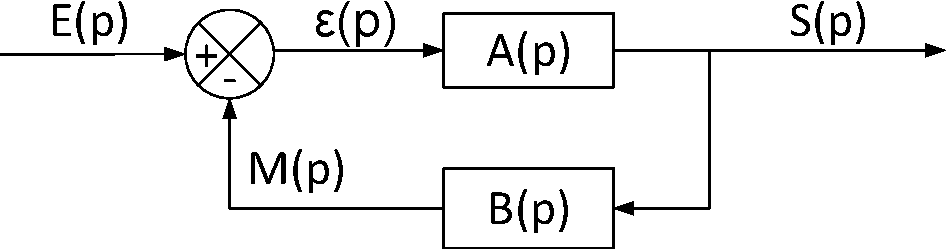
\includegraphics[width=0.8\linewidth]{img/fig10}
\end{minipage}\hfill
\begin{minipage}{0.55\linewidth}
 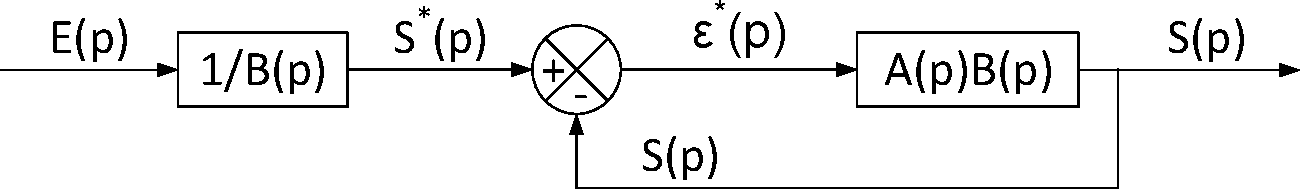
\includegraphics[width=0.8\linewidth]{img/fig11}
\end{minipage}

La fonction $\epsilon^*(p)$ mesure l'écart entre:
\begin{itemize}
 \item la réponse attendue (calculée à partir de la consigne d'entrée $E(p)$: $S^*(p)$,
 \item la réponse effective du système $S(p)$.
\end{itemize}

\vspace{-0.2cm}

\begin{center}
	$\epsilon^*(p)=S^*(p)-S(p)=S^*(p)-FTBF^*(p).S^*(p)=(1-FTBF^*(p)).S^*(p)$
\end{center}

\vspace{-0.2cm}

\begin{itemize}
 \item $FTBF^*(p)$ est la fonction de transfert en boucle fermée de la partie à retour unitaire,
 \item Elle peut s'écrire $FTBF^*(p)=\dfrac{FTBO(p)}{1+FTBO(p)}$.
\end{itemize} 
}}

{\frame{
\frametitle{Rapidité et précision en réponse à un échelon}

Si on suppose que l'entrée du système à retour unitaire est un échelon, on a :


\begin{center}
	$S^*(p)=\dfrac{S_0}{p}\rightarrow \epsilon^*(p)=(1-FTBF^*(p)).\dfrac{S_0}{p}$
\end{center}

Le théorème de la valeur finale permet de calculer la valeur de l'écart statique:

\begin{center}
$\epsilon^*(+\infty)=\lim\limits_{t \rightarrow +\infty} \epsilon^*(t)=\lim\limits_{p \rightarrow 0} p.\epsilon^*(p)=\dfrac{1}{1+FTBO(0)}.S_0$
\end{center}

Ainsi, si la FTBO du système est de classe 0, et quelque soit son ordre, le système ne peut pas atteindre la valeur finale commandée par la consigne en échelon de valeur. Il existe un écart statique donné par la relation: $\epsilon^*(+\infty)=\dfrac{S_0}{1+K}$ où $K$ est le gain statique du système en boucle ouverte.
}}

\section{Identification des S.L.C.I.}

 \ifdef{\public}{\begin{frame}
\frametitle{Table des matières}
\tableofcontents[currentsection]
\end{frame}}{}


{\frame{
\frametitle{Identification des S.L.C.I.}

\textbf{Modélisation et identification: Généralités}

~\

\begin{minipage}{0.7\linewidth}
\begin{itemize}
 \item La réalisation d'un asservissement d'une grandeur physique est la réponse à un besoin. Des critères d'appréciation de la fonction technique sont alors spécifiés en terme de rapidité, de précision, d'amortissement et parfois de stabilité,
 \item L'identification du modèle de comportement d'un SLCI est nécessaire afin de permettre de prévoir son comportement lors de son utilisation. Cette prévision permet de valider la solution retenue lors de la conception ou d'adapter sa correction afin qu'il réponde critère d'appréciation de la fonction technique,
\end{itemize}
\end{minipage}\hfill
\begin{minipage}{0.25\linewidth}
 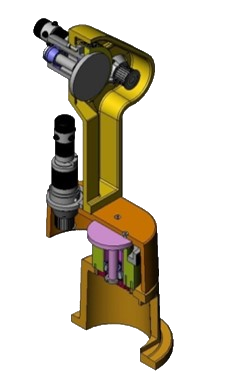
\includegraphics[width=0.8\linewidth]{img/fig12}
\end{minipage}

\begin{itemize}
 \item Un premier type d'approche consiste à établir un modèle physique du système que l'on doit valider. Il est appelé modèle de connaissance. Les paramètres physiques du système (résistance, inductance, masse, moment d'inertie) devant tous être calculés ou mesurés. 
\end{itemize}
}}

{\frame{
\frametitle{Identification des S.L.C.I.}

Exemple de modèle de connaissance d'un asservissement de vitesse d'un axe de robot

\begin{center}
 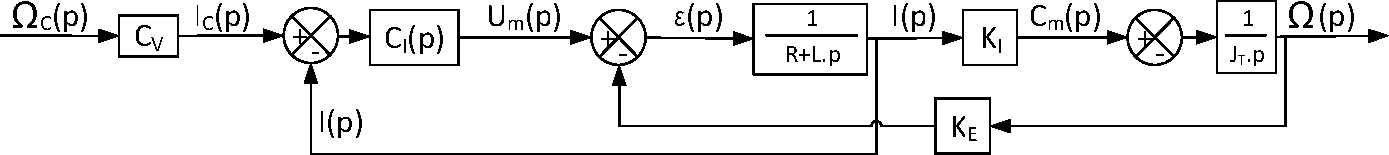
\includegraphics[width=0.9\linewidth]{img/fig13}
\end{center}

\begin{itemize}
 \item Ce type de modélisation nécessite donc l'identification de tous les paramètres physiques du modèle. Ceci est possible si la complexité du modèle n'est pas trop grande,
 \item Une deuxième méthode de modélisation est alors utilisée, c'est le modèle de représentation. On \textbf{postule} la forme simplifiée du modèle qui traduit le comportement déterminé expérimentalement. On \textbf{identifie}, en les ajustant, les paramètres de ce modèle simplifié pour qu'il traduisent le son comportement vis-à-vis d'une entrée déterminée. Ce type de modèle n'a pas de signification physique.
\end{itemize}
}}

{\frame{
\frametitle{Identification des S.L.C.I.: 1\up{er} ordre}

Pour identifier un modèle de représentation, nous nous limiterons à une entrée $e(t)$ de type échelon d'amplitude $E_0$. On note $s(t)$ la réponse mesurée du système. La fonction de transfert traduisant le modèle de représentation sera notée $H(p)$.

Système du \textbf{premier ordre} à constante de temps, il est caractérisé par une fonction de transfert du type :

\begin{minipage}{0.4\linewidth}
\begin{center}
$H(p)=\dfrac{K}{1+\tau.p}$
\end{center}
\end{minipage}\hfill
\begin{minipage}{0.55\linewidth}
\begin{center}
 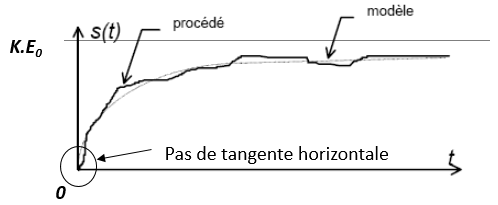
\includegraphics[width=0.9\linewidth]{img/fig14}
\end{center}
\end{minipage}

\begin{rem}
La réponse à un échelon se reconnaît par l'absence de tangente horizontale à l'origine.
\end{rem}
}}

{\frame{
\frametitle{Identification des S.L.C.I.: 1\up{er} ordre}

L'asymptote horizontale à l'infini permet de déterminer le gain statique $K$ à une constante multiplicative $E_0$ près.

\vspace{-0.5cm}

\begin{center}
 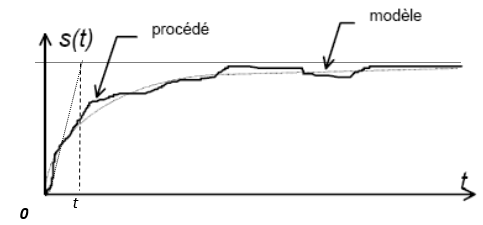
\includegraphics[width=0.4\linewidth]{img/fig15}
\end{center}

\vspace{-0.5cm}

La détermination de la constante de temps permet de confirmer la validité de cette modélisation. Le prolongement de la tangente à l'origine permet de déterminer la constante de temps $\tau$. Pour un signal bruité, il faut utiliser la valeur remarquable $0,63K$.

\begin{minipage}{0.4\linewidth}
\begin{itemize}
 \item Les valeurs pour $2.\tau$ et $3.\tau$ sont à vérifier,
 \item Vérifier également la cohérence du résultat vis-à-vis des tangentes.
\end{itemize}
\end{minipage}\hfill
\begin{minipage}{0.55\linewidth}
 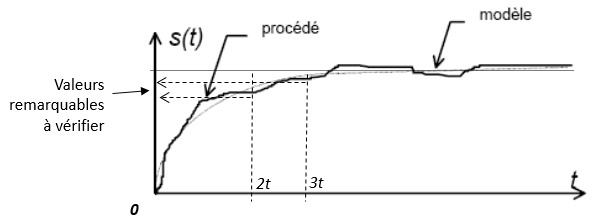
\includegraphics[width=0.9\linewidth]{img/fig16}
\end{minipage}
}}

{\frame{
\frametitle{Identification des S.L.C.I.: 2\up{ème} ordre}

Système du second ordre à pôles complexes conjugués, il est caractérisé par une fonction de transfert du type:

\begin{center}
$H(p)=\dfrac{K}{1+\dfrac{2.\xi}{\omega_0}+\left(\dfrac{p}{\omega_0}\right)^2}$	
\end{center}

\begin{itemize}
 \item Si $\xi>1$, la courbe se reconnait grâce à une tangente horizontale à l'origine,
 \item Si $\xi<1$, des pseudo-oscillations apparaissent.
\end{itemize}

\begin{center}
 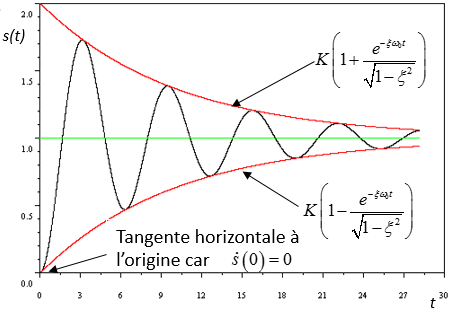
\includegraphics[width=0.45\linewidth]{img/fig17}
\end{center}
}}


{\frame{
\frametitle{Identification des S.L.C.I.: 2\up{ème} ordre}

L'identification des paramètres s'effectue à l'aide des relations suivantes.

\begin{itemize}
 \item La valeur du gain statique est donnée par : $s(+\infty)=K.E_0$,
 \item Le dépassement \% permet de déterminer la valeur du facteur d'amortissement $\xi$: \\
 \begin{center}
  $D\%=100.\dfrac{s_{max}-K.E_0}{K.E_0}=100.e^{-\xi.\dfrac{\pi}{\sqrt{1-\xi^2}}}$,
 \end{center}
 \item La pseudopériode $T_p$ est facilement identifiable. Il est possible alors d'utiliser le décrément logarithmique à partir d'un instant $t$ et pour $n$ pseudo-oscillations: \\
 \begin{center}
$\delta=Ln\left(\dfrac{s(t)}{s(t+n.T_p)}\right)=n.\dfrac{\xi.\pi}{\sqrt{1-\xi^2}}$,
 \end{center}
 \item A partir de la pseudo période $T_p$ et du facteur d'amortissement $\xi$, la valeur de $\omega_0$ ($s^{-1}$) peut être déduite : \\
  \begin{center}
  $\omega_0=\dfrac{2.\pi}{T_p.\sqrt{1-\xi^2}}$,
 \end{center}
 \item Le temps de réponse à 5\% peut être déduit de la courbe.
\end{itemize}
}}

{\frame{
\frametitle{Les systèmes asservis}

\begin{savoir}
Vous devez être capables :
\begin{itemize}
 \item De modéliser la structure d'un SLCI,
 \item D'identifier les réponses temporelles d'un SLCI.
\end{itemize}
\end{savoir}

\begin{prob}
Il est nécessaire d'utiliser d'autres types de sollicitations.
\begin{itemize}
 \item \textit{Problème: Quelle est la réponse harmonique d'un SLCI ?}
 \item \textbf{Perspectives}: Représenter la réponse d'un harmonique d'un système.
\end{itemize}
\end{prob}
}}

\end{document}